
\chapter{Gene regulation in space and time}
% \section{Transcription factor search}
% In chapter 2, we discussed the rate at which two molecules encounter each other by diffusion and derived the diffusion limit to association (see Eq.~\ref{eq:diffusion_limit}).
% To estimate the rate of transcription factor/DNA association, we can ignore the diffusion of DNA (it is a large slow molecule). Furthermore, the reaction radius should be of the same order as the distance between basepairs since the TFs recognize specific DNA sequences and hence have to be in register with the DNA to 0.3nm. Together with in-vitro measurements of diffusion constant of a transcription factor of about $100\mu m^2/s$, this results in a rate estimate
% \begin{equation}
% 	\kappa_{D} = 4\pi \times 100 \times 3\times 10^{-4} \mu m^3/s \approx 0.4  \mu m^3/s \approx 2\times 10^8 M^{-1}s^{-1}
% \end{equation}
% However, experiments have shown that the association rate is much higher!
% Furthermore, the association rate depends strongly on ionic strength, suggesting that unspecific electro-static interactions help in the binding site search.
% This conundrum, and potential solution, is discussed in the review by \citet{hippel_facilitated_1989}.

% The basic idea of the mechanisms by which association is sped up is the following:
% The TF associates with a random place on the DNA and starts to diffuse along the DNA for a while before detaching again, see Fig.~\ref{fig:TF_search}.
% This allows the TF to ``scan'' a section of the DNA in one dimension without having getting lost in 3D.
% The problem is hence characterized by a diffusion constant $D_{1D}$ along the DNA in 1D, a diffusion constant $D_{3D}$ in 3D, as well as the average times $\tau_{1D}$ and $\tau_{3D}$ spend in 1D and 3D.


% If combined 1D/3D diffusion was the mechanism by which TFs find their target, how should they be dividing their time between 3D and 1D search?
% Following \citep{mirny_how_2009}, the total time until the target is found can be expressed as the sum over multiple rounds of 3D/1D search
% \begin{equation}
% t_s = \sum_{i=1}^K (\tau_{1D,i} + \tau_{3D,i})
% \end{equation}
% and the typical number of rounds necessary would be $\bar{K} = L/l $ where L is the length of the genome and l is the length searched in a single round.
% Since $l\sim \sqrt{2D_{1D} \tau_{1D}}$, we obtain for the average search time
% \begin{equation}
%  t_s = \frac{L}{\sqrt{2D_{1D} \tau_{1D}} }(\tau_{1D}+\tau_{3D})
% \end{equation}
% The search time is minimal when
% \begin{equation}
%  \frac{d t_s}{d \tau_{1D}} = \frac{L}{2\sqrt{2D_{1D}}}(\tau_{1D}^{-1/2}-\tau_{3D}\tau_{1D}^{-3/2}) = 0
% \end{equation}
% which requires $\tau_{1D} = \tau_{3D}$, i.e., the TF should spend equal times on the DNA and in solution.
% The mean search time is therefore
% \begin{equation}
%  t_s = L\sqrt{\frac{2\tau_{3D}}{D_{1D}}}
% \end{equation}

% \begin{figure}[tb]
% 	\centering
% 	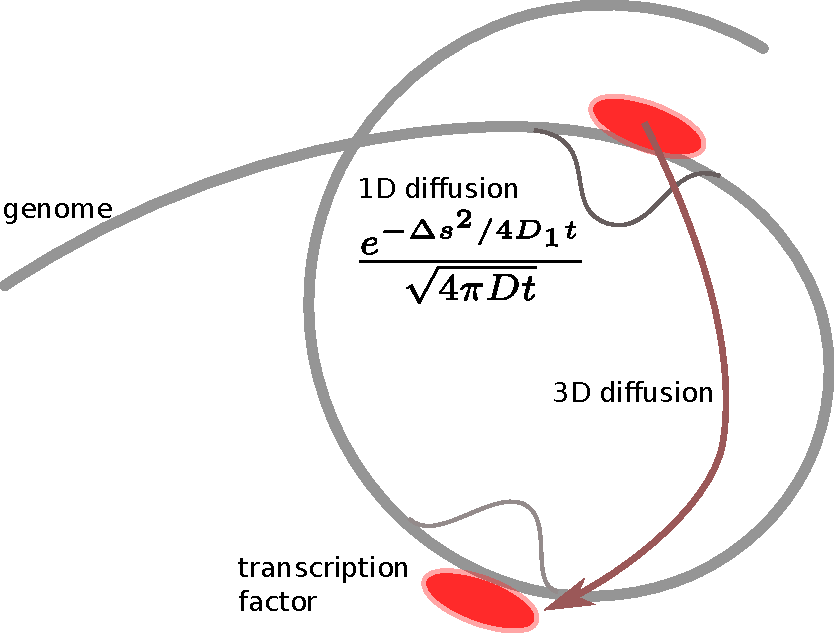
\includegraphics[width=0.7\textwidth]{TF_search.pdf}
% 	\caption{Illustration of combined 1D/3D search.}
% 	\label{fig:TF_search}
% \end{figure}

% \subsection*{Why is there an optimum?}
% One dimensional diffusion alone would be extremely inefficient since it takes very long time to scan the entire genome due to the square-root scaling of the distance covered.
% Very short $\tau_{1D}$, on the other hand, corresponds to very limited scanning of bases and in the limit of $\tau_{1D}\to 0$ corresponds to pure 3D search.
% Hence it is plausible that an optimum should exist.


Above, we have discussed models of cell-autonomous gene expression.
In the developing embryo, cells that are initially identical assume different fates and these fate decision are driven by the differential expression of genes.
The gene expression programs are controlled in space and time through the diffusion of signaling molecules or transcription factors and mechanical coupling of different parts of the embryo.
A paradigmatic example of spatial gene regulation through spatially spreading transcription factors is the activation of the gene \emph{hunchback} in the early Drosophila embryo.
For a short introduction into early Drosophila development, have a look at \url{https://youtu.be/Ncxs21KEj0g}.

\begin{figure}[tb]
	\centering
	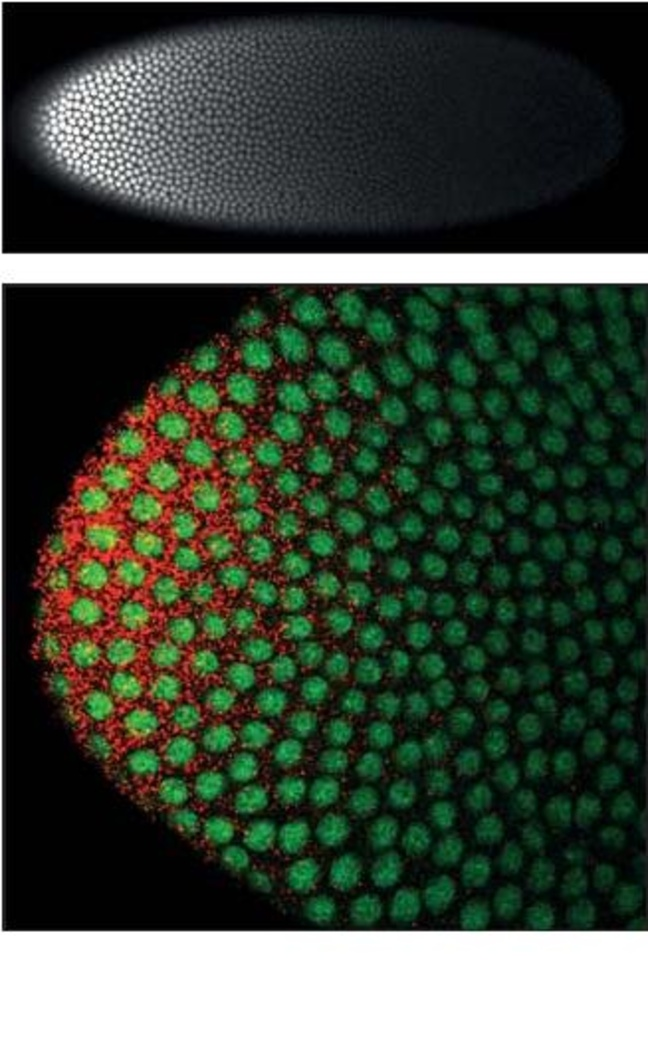
\includegraphics[width=0.3\textwidth]{figures/Fluorescent_labeling_of_Bicoid_GFP_and_mRNA.jpg}
	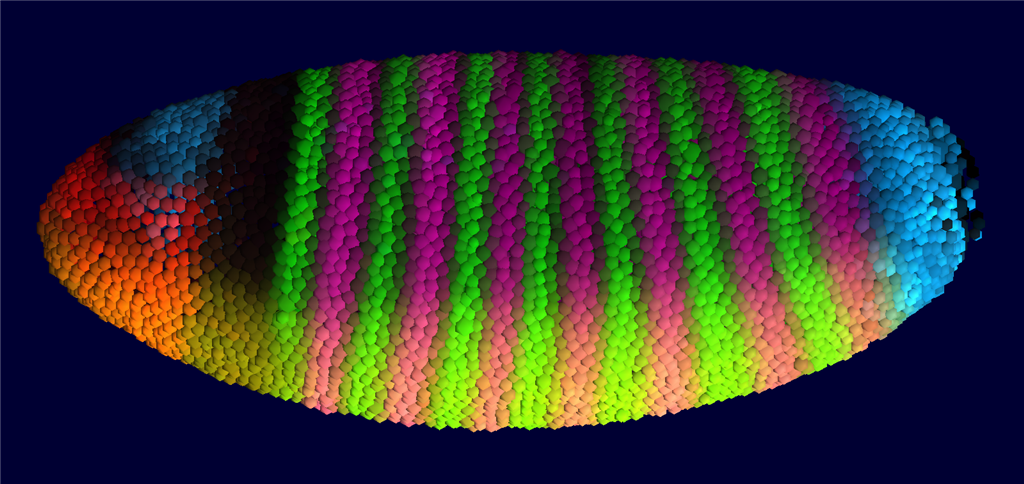
\includegraphics[width=0.68\textwidth]{figures/fly_embryo.png}
	\caption{Left: Bicoid gradient (top) and RNA localisation (in red) in the lower panel (by Thomas Gregor, Julien O. Dubuis, Shawn C. Little).
	Right: Computational synthesis of gene expression patters in the fly embryo (from \url{https://dav.lbl.gov/archive/Events/SC05/Drosophilia/index.html}).
	}
	\label{fig:fly_gene_expression}
\end{figure}

Fig.~\ref{fig:fly_gene_expression} shows the earliest pattern -- the bicoid gradient --  on the left and a later more elaborate pattern of gene expression on the right.
As an example, we want to discuss the generation of the bicoid gradient and the resulting of {\it hunchback}.
The gene {\it hunchback} is expressed in the half of the cell with higher bicoid concentration with a very sharp boundary between cells that express it at full strength and those that don't: cells ``read'' the bicoid concentration and depending on whether this concentration is larger than a threshold, they express the target.
We will ask two questions: How is such a gradient established? And how is it read out?


\subsection*{Gradient formation by diffusion and decay}
Bicoid is produced at one end of the embryo through translation of mRNA that was deposited there by the mother.
The protein diffuses away from that pole through embryo.
That alone would slowly result in a homogeneous concentration of bicoid.
Bicoid, however, is unstable and degradation of bicoid coupled with diffusion results in a gradient.

For the purposes of studying the gene expression gradient, we only need to consider the long axis of the embryo, that it is sufficient to model the bicoid profile in one dimension.
Analogously to our discussion in chapter two (Eq.~\ref{eq:discrete_update}), we begin with a discrete one-dimensional model with spatial bins of width $\Delta x$, see Fig.~\ref{fig:reaction_diffusion}.
The concentration $b_i$ of bicoid in bin $i$ changes according to
\begin{equation}
	b_i(t+dt) = \delta_{i0}\alpha dt + (1-\beta dt )b_i + dt\frac{D}{\Delta x^2} (b_{i-1} - 2b_i + b_{i+1})
\end{equation}
Here $\beta dt$ is the fraction of bicoid that decays in a time interval $dt$, $\delta_{i0}\alpha dt$ is the production of bicoid that only happens in bin $i=0$, and the last term describes the discretized diffusion.
In analogy to Eq.~\ref{eq:diffusion}, this discrete equation is rewritten as a differential equation
\begin{equation}
	\frac{\partial b(x,t)}{\partial t} = \delta(x)\alpha + D\frac{\partial^2 b(x,t)}{\partial x^2} - \beta b(x,t)
\end{equation}
The ``delta-function'' $\delta(x)$ is a spike at $x=0$ and vanishes everywhere else.
This term models the production of bicoid at the very left end of the embryo.
The second term is the familiar diffusion term, while the last term models the degradation of bicoid with rate $\beta$.

We are interested in a steady state solution for $b(x,t)$ and we will first solve this equation for $x>0$ where the production term is absent.
Setting $\frac{\partial b(x,t)}{\partial t}=0$, we have for $x>0$
\begin{equation}
b(x) = \frac{D}{\beta}\frac{\partial^2 b(x)}{\partial x^2}
\end{equation}
This equation has the solution $b(x) = a e^{-\sqrt{\frac{\beta}{D}}x}$, i.e., the steady state concentration profile is an exponential decay with length scale $\ell = \sqrt{D/\beta}$.
The decay rate $\beta$ is the inverse of the bicoid life time $\tau = 1/\beta$ and the decay length can hence be rewritten as $\ell = \sqrt{D \tau}$.
The distance over which bicoid spreads from its source is hence given by a trade-off between diffusion and decay: The longer the protein lives, the shallower is the gradient.
And the scaling makes sense: after a typical lifetime $\tau$, we expect the bicoid to have moved a net distance of about $\sqrt{D\tau}$.

We can account for the production term by imposing a flux $\alpha$ through the boundary at $x=0$.
The flux is $-D\frac{\partial b(x)}{\partial x}|_{x=0}=a \sqrt{D\beta}=\alpha$ and therefore $a = \alpha/\sqrt{D\beta}$.
The full steady state solution is therefore
\begin{equation}
 	b(x) = \alpha \sqrt{\frac{\tau}{D}} e^{-x/\sqrt{D\tau}}
\end{equation}
Numerical solution of the discrete system agrees well with this analytical steady state solution, see Fig.~\ref{fig:reaction_diffusion}B.

\begin{figure}[tb]
	\centering
	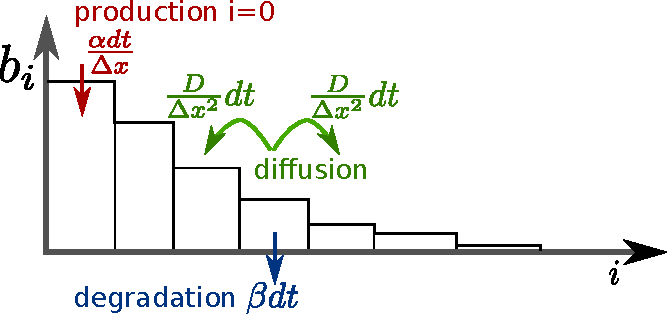
\includegraphics[width=0.48\textwidth]{reaction_diffusion.pdf}
	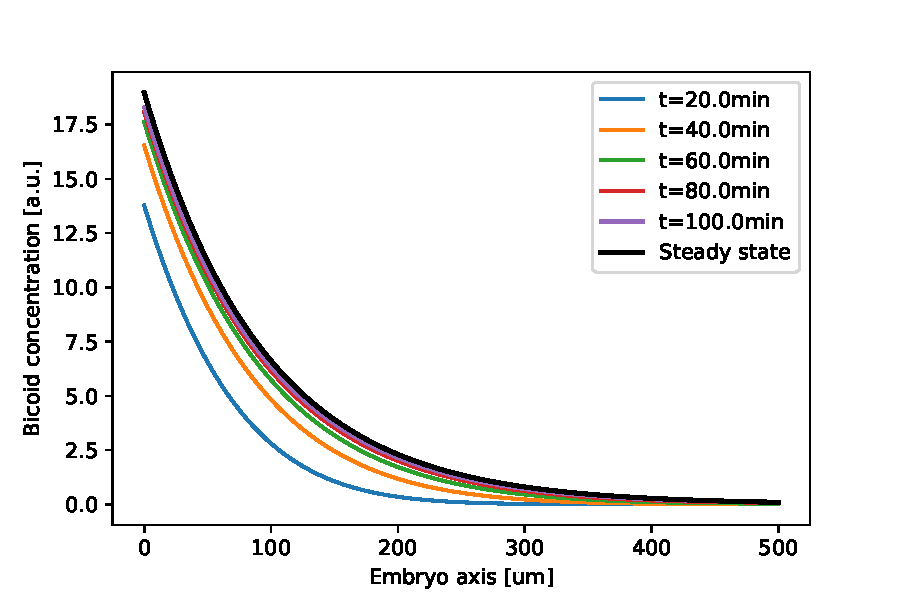
\includegraphics[width=0.48\textwidth]{figures/bicoid_gradient.pdf}
	\caption{Left: Discrete model of the reaction diffusion system governing the bicoid gradient.
	Right: Numerical solution of the discrete reaction diffusion equation and the analytical steady state solution.}
	\label{fig:reaction_diffusion}
\end{figure}

In a developing fly embryo, it seems that diffusion of bicoid is not simply a random walk of the molecule, but facilitated by large-scale back and forth movements of the cytosol during successive cycles of cell division.
For an overview of recent research on that topic, have a look at the online presentation by Eric Wieschaus at \href{https://youtu.be/cpOf5el9GIk}{youtu.be/cpOf5el9GIk}.

Careful fluorescence microscopy measurements of GFP-tagged Bicoid have shown that the gradient builds up over a scale of 2 hours and is extremely reproducible from one embryo to the next, see Fig.~\ref{fig:bicoid_gradient}.
This reproducibility is important to ensure the accurate separation of the embryo into anterior and posterior half.
This behavior can be quantitatively described by the reaction diffusion model discussed above.

\begin{figure}[tb]
	\centering
	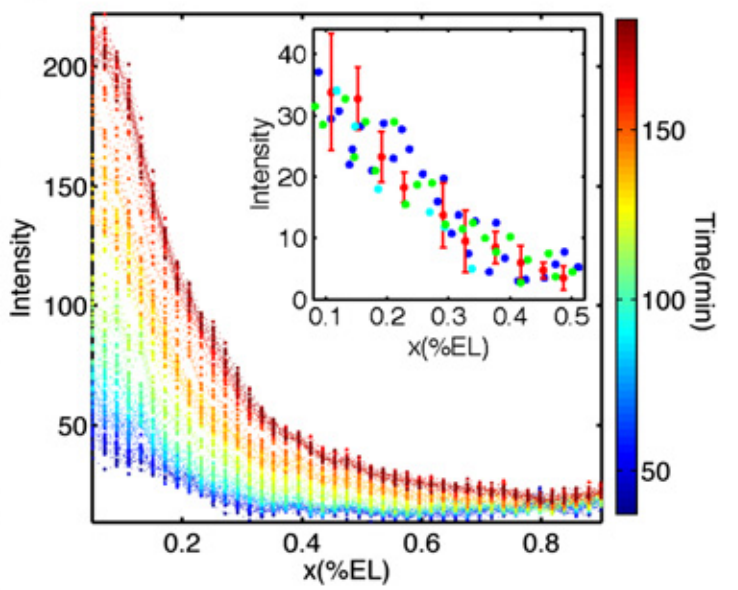
\includegraphics[width=0.43\textwidth]{figures/Gregor_Bcd_gradient_buildup.png}
	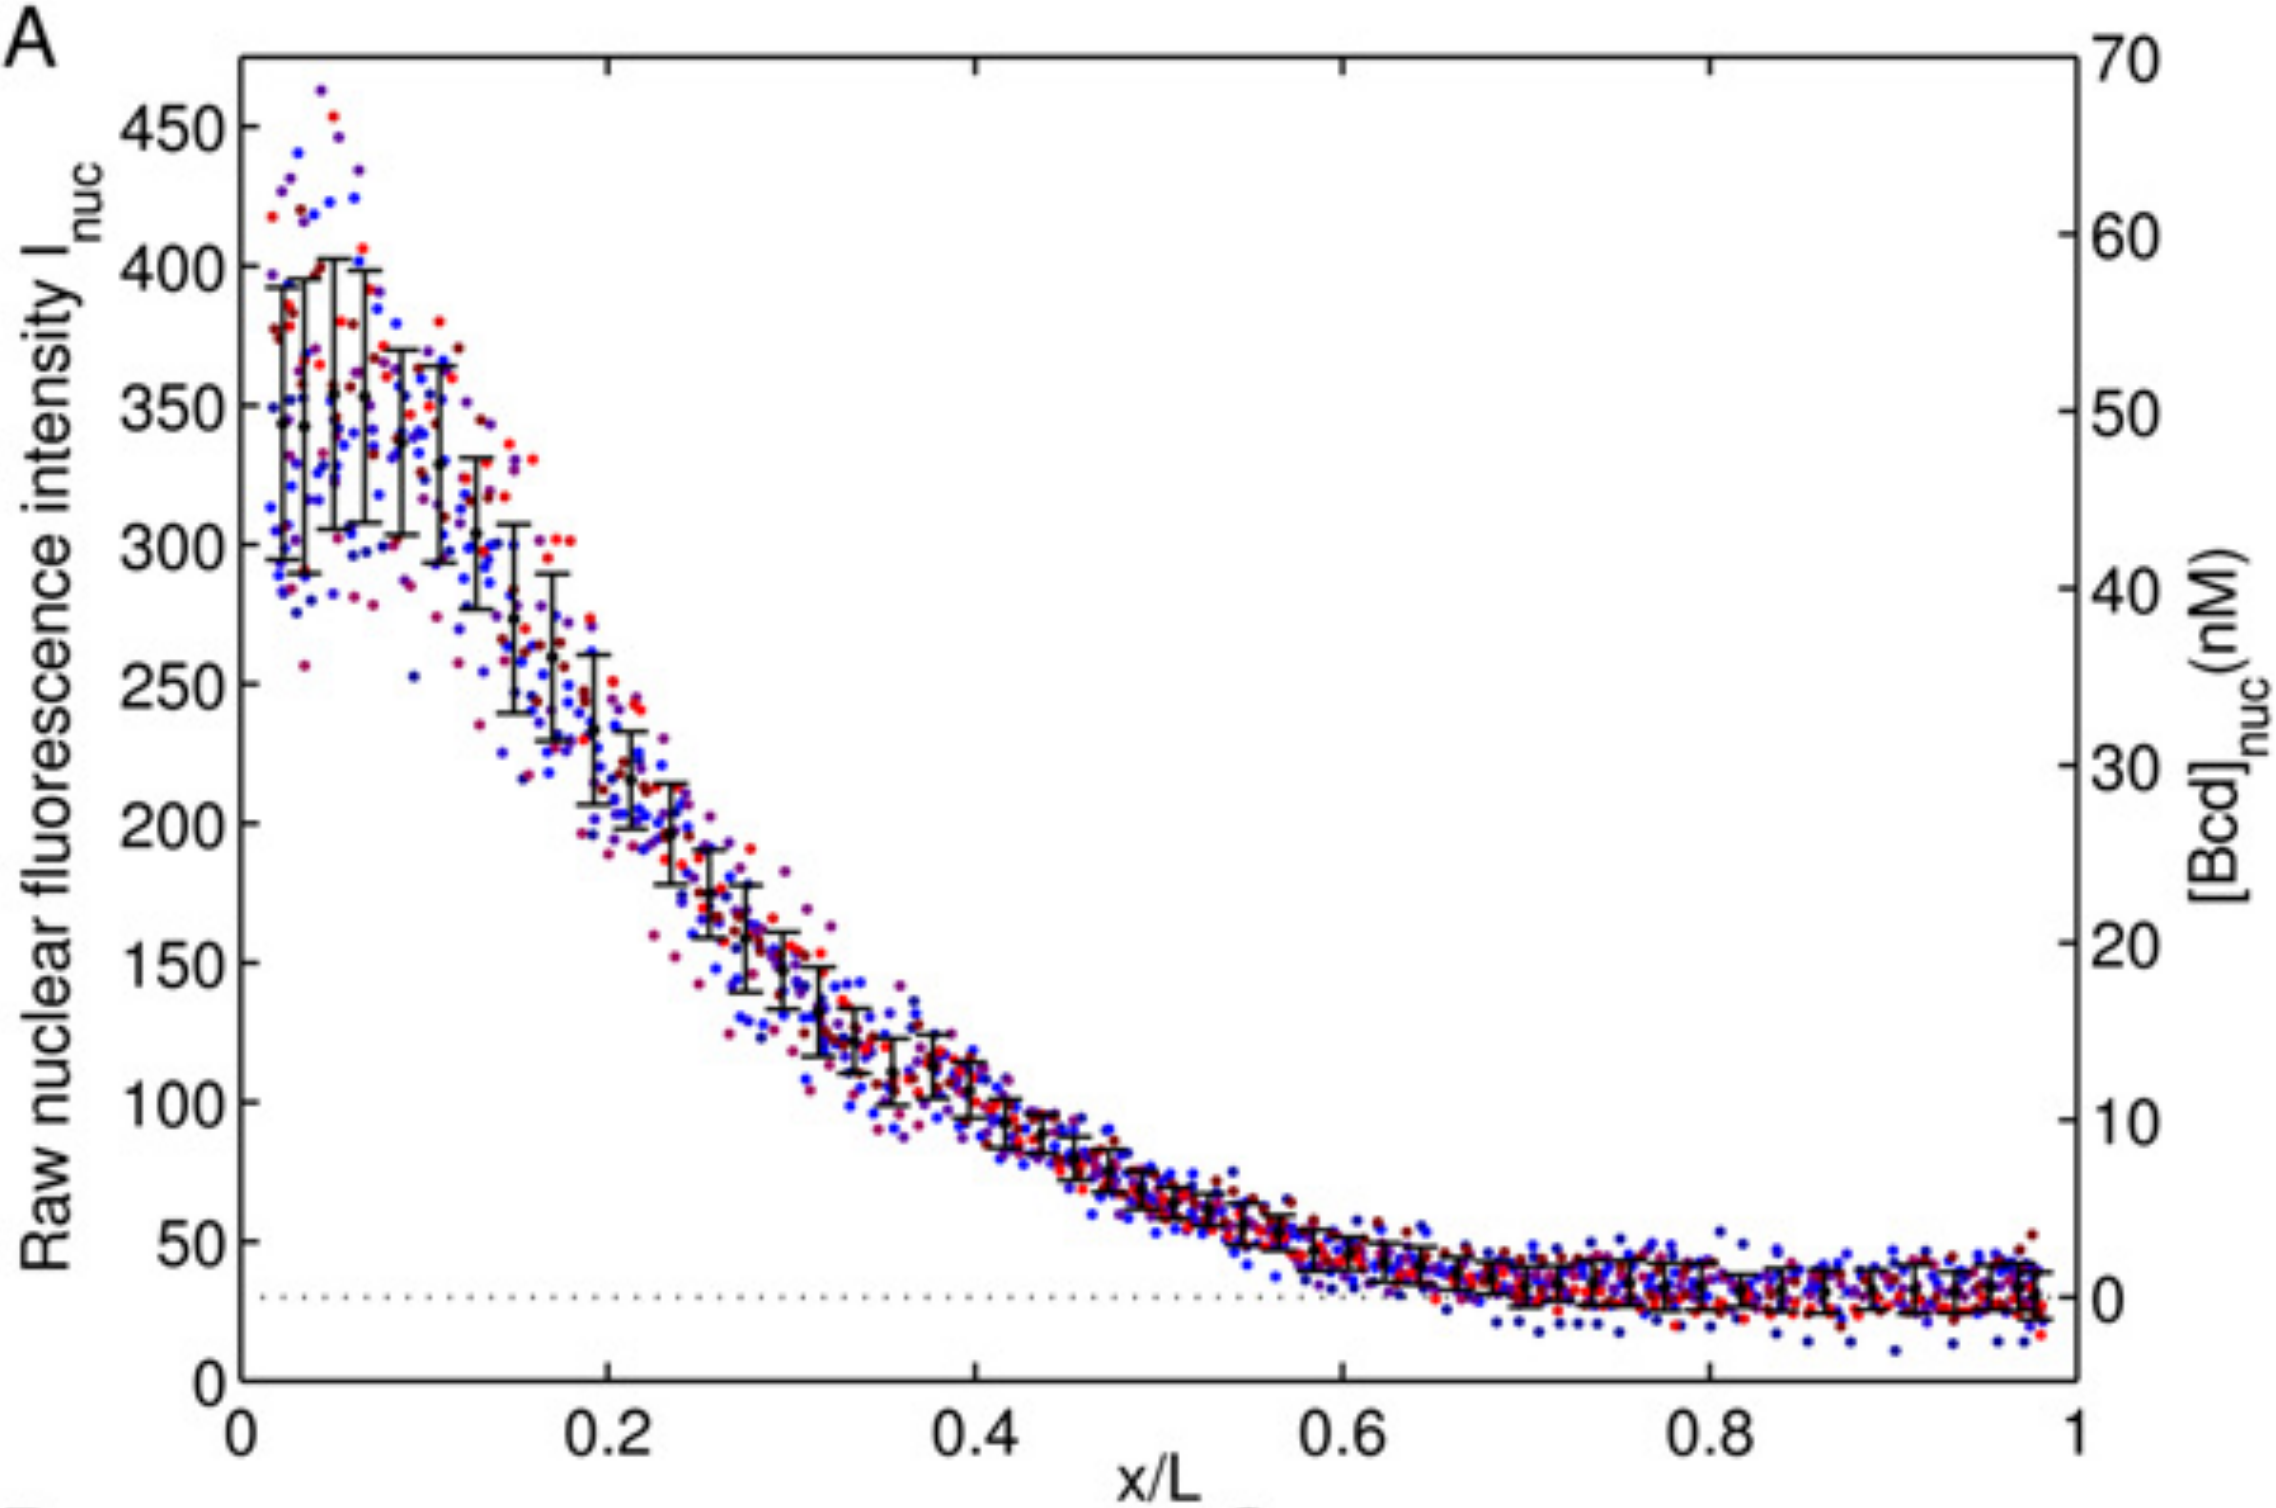
\includegraphics[width=0.55\textwidth]{figures/Gregor_Bcd_gradient_reproducibility.png}
	\caption{Experimental characterization of the Bicoid gradient: Left) The gradient establishes itself over a time span of about 2 hours. Right: Different embryos have very similar Bicoid gradients at nuclear cycle 14. From \citep{gregor_stability_2007} and \citep{gregor_probing_2007}.}
	\label{fig:bicoid_gradient}
\end{figure}


\section{Patterning with reaction diffusion systems}
Reaction diffusion systems can generate much more interesting patterns than the gradient discussed above.
If two or more diffusion species interact, the result could be stationary patterns with spots or strips as well as dynamic wave-like patterns.
Many biological patterns (Zebra strips, leopard dots, etc) are believed to have their origin in such systems.
The best known such patters are {\it Turing patterns}.
\href{https://en.wikipedia.org/wiki/Alan_Turing}{Alan Turing} was a British mathematician who made many seminal contributions to computer science.
In addition, he showed that two-species reaction diffusion systems naturally generate many patterns common in biology \citep{turing_chemical_1952}.
These system have the general form
\begin{eqnarray}
	\frac{\partial u(x,t)}{\partial t} &=& D_u \frac{\partial^2 u(x,t)}{\partial x^2} + f(u(x,t),v(x,t)) \\
	\frac{\partial v(x,t)}{\partial t} &=& D_v \frac{\partial^2 v(x,t)}{\partial x^2} + g(u(x,t),v(x,t))
\end{eqnarray}
Often these systems are formulated in two dimensions, were they generate 6 distinct possible behaviors depending on the parameters and how the two species interact.
One class of these solutions forms stable patterns that often look very similar to patterns that one observes across the animal kingdom \citep{kondo_reaction-diffusion_2010}.

The basic mechanism of Turing patterns is often summarized as {\it short-range activation -- long-range inhibition}.
Both substances inhibit each others production and enhance their own production.
By tuning the ratios of diffusion constants, different types of patterns can be generated.

\begin{figure}[tb]
	\centering
	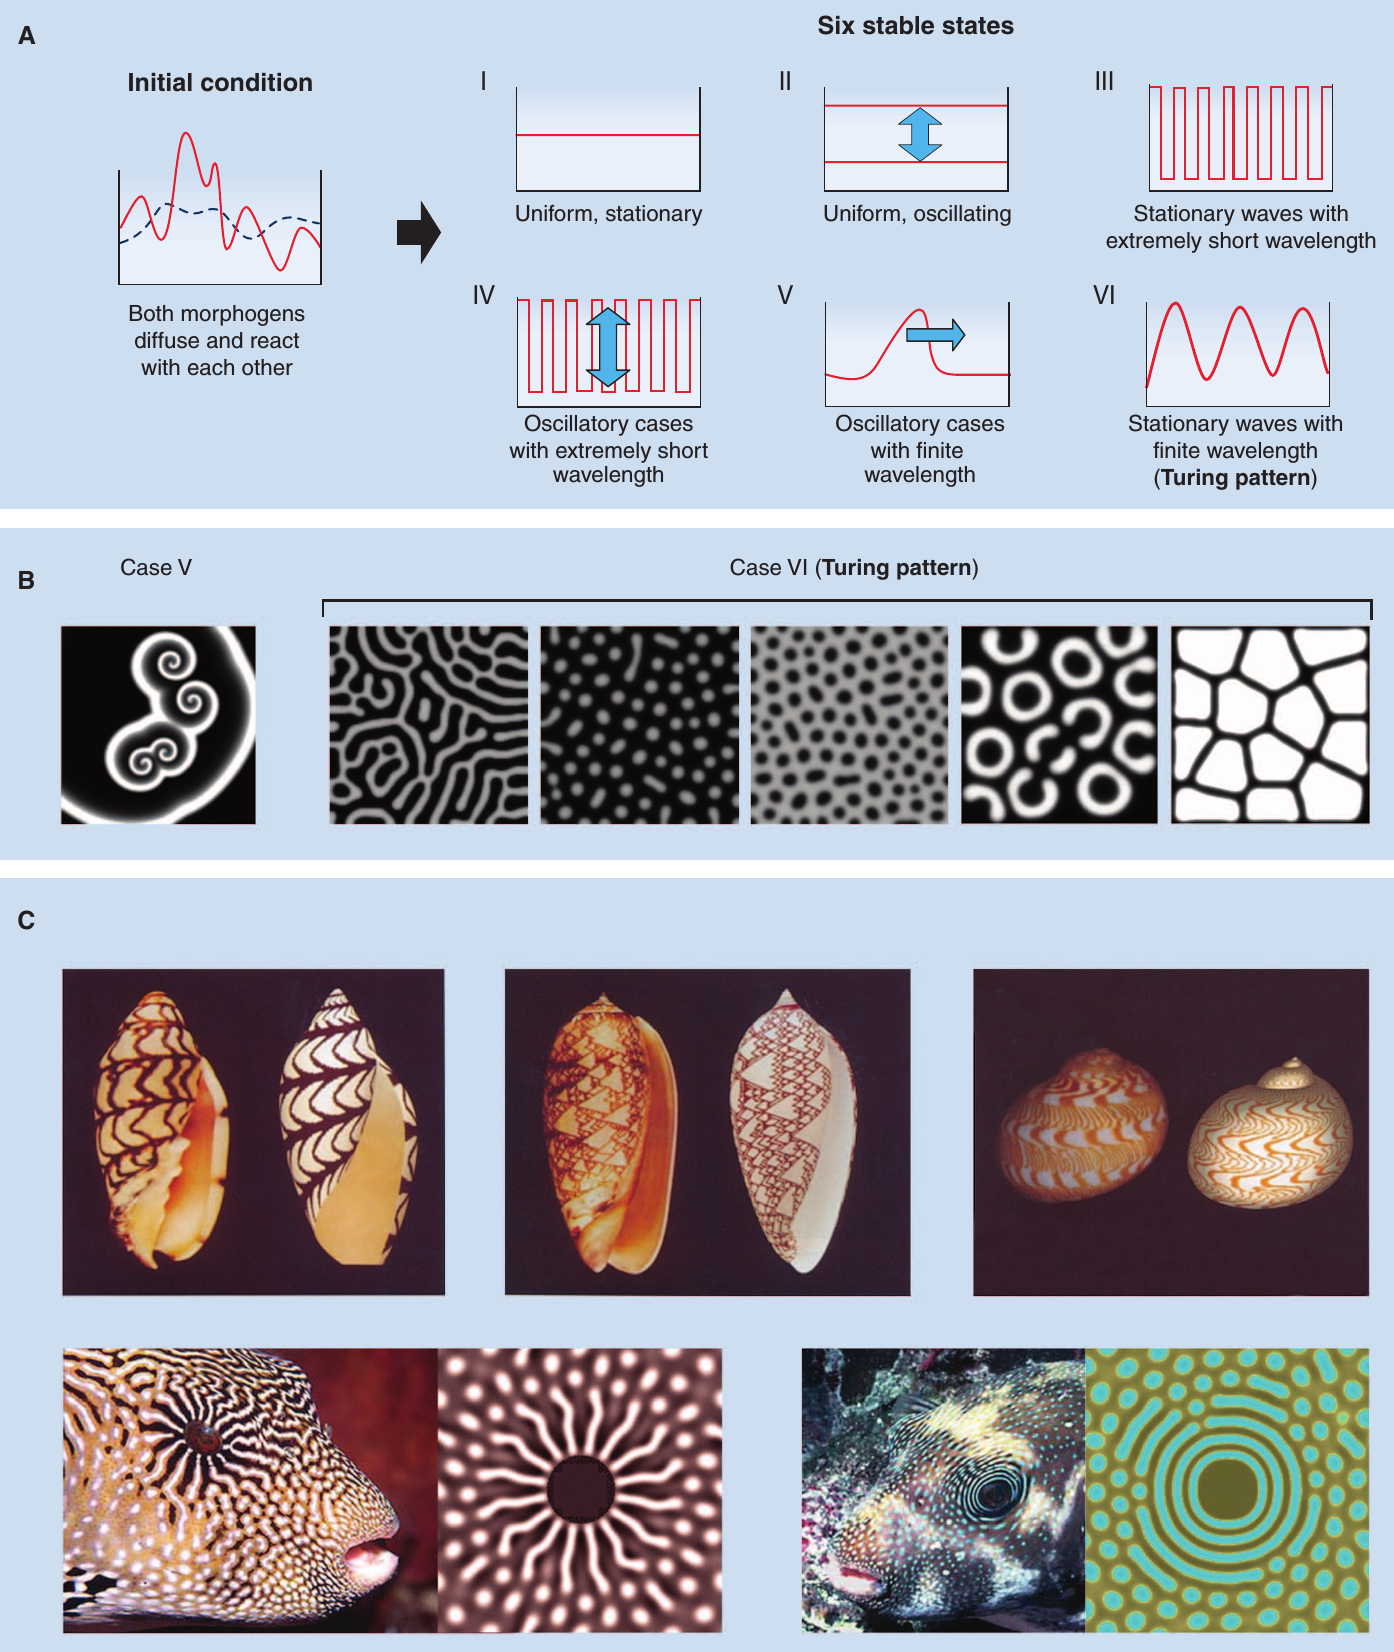
\includegraphics[width=0.98\textwidth]{figures/Kondo_Turing_patterns.png}
	\caption{Turing patterns. A) The generic states of a homogeneous reaction-diffusion system. B) Case V corresponds to traveling waves that often form spirals. The classical Turing patterns (Case VI) consist of stripes, dots, and domains for different parameters.
	C) These patterns are often very reminiscent of patterns observed in biology.
	From \citep{kondo_reaction-diffusion_2010}.}
	\label{fig:turing}
\end{figure}

